\section{Evaluation}
\label{sec:evaluation}

In this section, we present a comprehensive evaluation of \sysname, covering overall training performance (\S\ref{sec:evaluation:performance}), ablation studies of \sysname's key optimizations (\S\ref{sec:evaluation:ablation}), and the effectiveness of the precision-communication co-design (\S\ref{sec:evaluation:co-design}). Table~\ref{tab:evaluation:model_conf} lists the configurations of the MoE models used in our evaluation, detailing hidden size ($h$), FFN intermediate size ($h_{ffn}$), number of experts, and top-$k$ values. 
The evaluation is conducted on NVIDIA H800 GPUs unless otherwise specified, with the specifications provided in Table~\ref{tab:evaluation:gpu_spec}. 

\begin{table}[t!]
    \centering
    \resizebox{\linewidth}{!} {
        \begin{tabular}{c|c|c|c|c}
            \hline
            \hline
            \multirow{2}{*}{\begin{tabular}[c]{@{}c@{}}System\end{tabular}} & \multirow{2}{*}{\begin{tabular}[c]{@{}c@{}}\#GPUs\end{tabular}} & \multirow{2}{*}{\begin{tabular}[c]{@{}c@{}}Iteration\\ Time (s)\end{tabular}} & \multirow{2}{*}{\begin{tabular}[c]{@{}c@{}}Throughput\\ (tokens/s)\end{tabular}} & \multirow{2}{*}{\begin{tabular}[c]{@{}c@{}}Training Time for\\ 1T Tokens (days)\end{tabular}} \\
            & & & & \\\cline{1-5}
            \multirow{5}{*}{Megatron-LM} & 240 & 39.94 & 151.1k & 76.61 \\
            & 480 & 19.56 & 301.1k & 38.38 \\
            & 720 & 13.70 & 430.5k & 26.88 \\
            & 960 & 10.82 & 550.2k & 21.23 \\
            & 1440 & 7.90 & 746.6k & 15.50 \\\cline{1-5}
            \multirow{5}{*}{\sysname} & 240 & 21.61 & 272.9k (\textbf{1.81$\times$}) & 42.41 \\
            & 480 & 11.83 & 498.6k (\textbf{1.65$\times$}) & 23.21 \\
            & 720 & 7.97 & 740.1k (\textbf{1.72$\times$}) & 15.64 \\
            & 960 & 6.12 & 963.8k (\textbf{1.77$\times$}) & 12.01 \\
            & 1440 & 4.19 & 1407.7k (\textbf{1.88$\times$}) & 8.22 \\
            \hline
            \hline
        \end{tabular}
    }
    % \vspace{-0.1in}
    \caption{Strong-scaling training performance for the 352B MoE model with NVIDIA H800 GPUs. The number in parentheses in the throughput column represents the speedup of \sysname compared to Megatron-LM.}
    \vspace{-0.2in}
    \label{tab:evaluation:strong-scaling}
\end{table}

\subsection{Training Performance}
\label{sec:evaluation:performance}

\sysname is built on top of Megatron-LM~\cite{shoeybi2019megatron}, a state-of-the-art open-source LLM training system that supports 3D parallelism strategies and is continuously updated to incorporate the latest optimizations from the community. Our evaluation uses the Megatron-LM on GitHub~\cite{megatron-lm} with commit hash f1f03922, selected for its stability at the commencement of our experiments months ago. For fair comparison, we use the same global batch size for Megatron-LM and \sysname and choose the optimal parallelism configurations for the two systems, respectively. Specifically, \sysname employs SP attention and EP within each node, while Megatron-LM adopts TP within each node, with both systems configured with a PP size of 15. \revision{We tune the configuration of Megatron-LM to meet its requirement of a uniform TP size across all components. As discussed in \S\ref{sec:design:parallelism:sp_attention}, for Megatron-LM, a TP size of 1 leads to a prohibitive 8$\times$ activation memory (addressable only with slow recomputation via gradient checkpointing), while a TP size of 8 forces EP to operate across nodes, incurring more communication costs than PP. Notably, both systems in the evaluation enable the communication-computation overlap techniques from MegaScale~\cite{jiang2024megascale} for data and pipeline parallelism. Therefore, the communication overhead mainly comes from intra-node model parallelism, e.g. TP, SP and EP.} Sequence length is 8,192 and vocabulary size is 65,536. 
% \todo{Can we mention the hardware used in the experiments? e.g., Hopper GPUs? Unclear what GPUs Table 3 and Figure 11 use. Only Figure 12 has the GPU types.}

% \begin{table}[t!]
%     \centering
%     \resizebox{\linewidth}{!} {
%         \begin{tabular}{c|c|c|c|c}
%             \hline
%             \hline
%             \multirow{2}{*}{\begin{tabular}[c]{@{}c@{}}System\end{tabular}} & \multirow{2}{*}{\begin{tabular}[c]{@{}c@{}}\#GPUs\end{tabular}} & \multirow{2}{*}{\begin{tabular}[c]{@{}c@{}}Iteration\\ Time (s)\end{tabular}} & \multirow{2}{*}{\begin{tabular}[c]{@{}c@{}}Throughput\\ (tokens/s)\end{tabular}} & \multirow{2}{*}{\begin{tabular}[c]{@{}c@{}}MFU\end{tabular}} \\
%             & & & & \\\cline{1-5}
%             \multirow{5}{*}{Megatron-LM} & 240 & 39.94 & 151.1k & 17.98\% \\
%             & 480 & 19.56 & 301.1k & 17.94\% \\
%             & 720 & 13.70 & 430.5k & 17.08\% \\
%             & 960 & 10.82 & 550.2k & 16.22\% \\
%             & 1440 & 7.90 & 746.6k & 14.81\% \\\cline{1-5}
%             \multirow{5}{*}{\sysname} & 240 & 21.61 & 272.9k & 32.48\%(\textbf{1.81$\times$}) \\
%             & 480 & 11.83 & 498.6k & 29.67\% (\textbf{1.65$\times$}) \\
%             & 720 & 7.97 & 740.1k & 29.36\% (\textbf{1.72$\times$}) \\
%             & 960 & 6.12 & 963.8k & 28.67\% (\textbf{1.77$\times$}) \\
%             & 1440 & 4.19 & 1407.7k & 27.89\% (\textbf{1.88$\times$}) \\
%             \hline
%             \hline
%         \end{tabular}
%     }
%     % \vspace{0.05in}
%     \caption{Strong-scaling training performance for the 352B MoE model, with a global batch size of 720 for all experiments. The number in parentheses in the MFU column represents the speedup of \sysname compared to Megatron-LM.}
%     \vspace{-0.15in}
%     \label{tab:evaluation:strong-scaling}
% \end{table}

% \begin{table*}[t!]
%     \centering
%     \resizebox{\linewidth}{!} {
%         \begin{tabular}{c|c|c|c|c|c|c}
%             \hline
%             \hline
%             \multirow{2}{*}{\begin{tabular}[c]{@{}c@{}}Batch Size\end{tabular}} & \multirow{2}{*}{\begin{tabular}[c]{@{}c@{}}System\end{tabular}} & \multirow{2}{*}{\begin{tabular}[c]{@{}c@{}}\#GPUs\end{tabular}} & \multirow{2}{*}{\begin{tabular}[c]{@{}c@{}}Iteration Time (s)\end{tabular}} & \multirow{2}{*}{\begin{tabular}[c]{@{}c@{}}Throughput\\ (tokens/s)\end{tabular}} & \multirow{2}{*}{\begin{tabular}[c]{@{}c@{}}MFU\end{tabular}} & \multirow{2}{*}{\begin{tabular}[c]{@{}c@{}}Aggregated\\ PFlops/s\end{tabular}}  \\
%             & & & & & & \\\cline{1-7}
%             \multirow{10}{*}{720} 
%             & \multirow{5}{*}{Megatron-LM} & 240 & 39.94 & 151.1k & 17.98\% & 42.68 \\
%             &  & 480 & 19.56 & 301.1k & 17.94\% & 85.16 \\
%             &  & 720 & 13.70 & 430.5k & 17.08\% & 121.62 \\
%             &  & 960 & 10.72 & 550.2k & 16.37\% & 155.42 \\
%             &  & 1440 & 7.90 & 746.6k & 14.81\% & 210.92 \\\cline{2-7}
%             & \multirow{5}{*}{\sysname} & 240 & 21.61 & 272.9k & 32.48\%(\textbf{1.81$\times$}) & 77.09 \\
%             &  & 480 & 11.83 & 498.6k & 29.67\% (\textbf{1.65$\times$}) & 140.85 \\
%             &  & 720 & 7.97 & 7401.k & 29.36\% (\textbf{1.72$\times$}) & 209.07 \\
%             &  & 960 & 6.12 & 963.8k & 28.67\% (\textbf{1.75$\times$}) & 272.20 \\
%             &  & 1440 & 4.19 & 1407.7k & 27.89\% (\textbf{1.88$\times$}) & 397.20 \\
%             \hline
%             \hline
%         \end{tabular}
%     }
%     \caption{Strong-scaling training performance for the 352B MoE model. The number in parentheses in the MFU column represents the speedup of \sysname compared to Megatron-LM. \todo{More details in the title. Refer to MegaScale.}}
%     \vspace{-0.15in}
%     \label{tab:evaluation:scalability}
% \end{table*}

\begin{figure}[t!]
    \centering
    
\includegraphics[width=0.8\linewidth]{figures/eval/weak_scaling.pdf}
    \vspace{-0.15in}
    \caption{Weak-scaling training performance for the 352B MoE model with NVIDIA H800 GPUs.}
    \vspace{-0.1in}
    \label{fig:eval:weak-scaling}
\end{figure}

\parabf{Scalability.} Table~\ref{tab:evaluation:strong-scaling} compares the strong-scaling training performance of Megatron-LM and \sysname on the 352B MoE model. We scale the number of GPUs while keeping the global batch size fixed at 720. 
% This experimental setting is more realistic, given that batch size is constrained by convergence effects and cannot be indefinitely scaled with the number of GPUs. 
Across all settings, \sysname achieves 1.65–1.88$\times$ speedups over Megatron-LM. As the number of GPUs increases, the MFU (Model FLOPs Utilization) of \sysname declines from 32.48\% to 27.89\%. This is expected, as the batch size is fixed and the number of micro-batches for each pipeline decreases with more GPUs, leading to more bubbles. 

Figure~\ref{fig:eval:weak-scaling} presents the weak-scaling training performance of Megatron-LM and \sysname on the same model. We scale the global batch size from 360 to 1,080 in proportion to the number of GPUs (from 480 to 1,440). \sysname achieves a 1.74-1.79$\times$ training throughput compared to Megatron-LM. As the scale increases, Megatron-LM’s throughput degrades by 2.74\% due to increased communication overhead. In contrast, \sysname exhibits near-linear scalability, with its throughput declining by only 0.2\%, benefiting from comprehensive communication-computation overlap. 
% \sysname achieves a 12.67\% higher MFU than Megatron-LM. As the scale increases, Megatron-LM’s MFU drops by 0.46\% due to increased communication overhead, whereas \sysname exhibits near-linear scalability, benefiting from comprehensive communication overlap. 

\begin{figure}[t!]
    \centering
    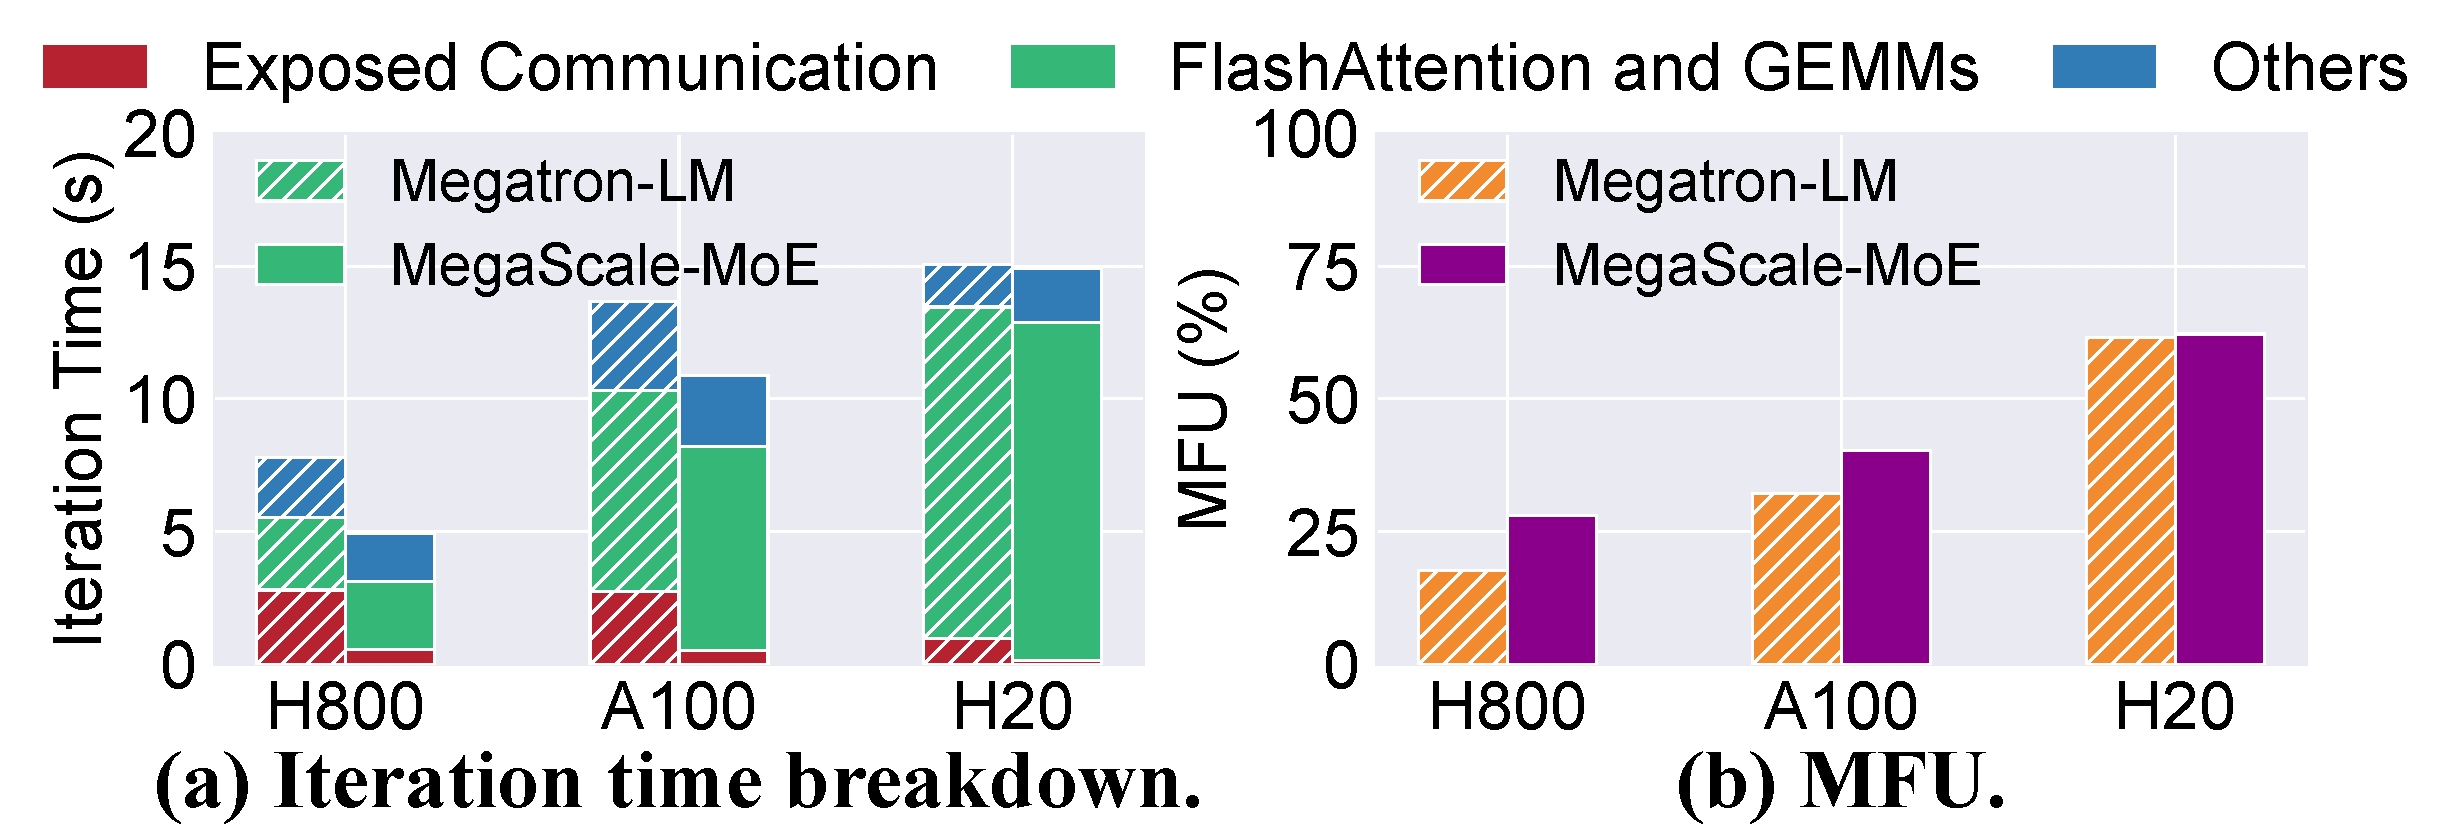
\includegraphics[width=\linewidth]{figures/eval/different_gpus.pdf}
    \vspace{-0.3in}
    \caption{Performance breakdown of training Mixtral-8$\times$7B on different GPUs.}
    \vspace{-0.1in}
    \label{fig:eval:different_gpus}
\end{figure}

\begin{table}[t!]
    \centering
    \resizebox{0.9\linewidth}{!} {
        \begin{tabular}{c|c|c|c|c}
            \hline
            % \hline
            \multirow{2}{*}{GPU} & 
            \multirow{2}{*}{\begin{tabular}[c]{@{}c@{}}Compute Cap-\\ability (TFLOPS)\end{tabular}} & 
            \multicolumn{2}{c|}{Memory Spec.} & 
            \multirow{2}{*}{\begin{tabular}[c]{@{}c@{}}NVLink\\ Bw. (GB/s)\end{tabular}} \\
            \cline{3-4}
            & & Cap. (GB) & Bw. (TB/s) & \\
            \hline
            H800 & 989 & 80 & 3.4 & 400 \\
            A100 & 312 & 80 & 2.0 & 600 \\
            H20 & 148 & 96 & 4.0 & 900 \\
            \hline
            % \hline
        \end{tabular}
    }
    % \vspace{-0.1in}
    \caption{Specifications of different NVIDIA GPUs.}
    \vspace{-0.15in}
    \label{tab:evaluation:gpu_spec}
\end{table}

\parabf{Performance breakdown on different GPUs.} We conduct a deep dive into \sysname to further understand the performance of training a MoE model in production environments. We train Mixtral-8$\times$7B on 32 NVIDIA H800, H20, and A100 GPUs, respectively. The specifications of GPUs we used are listed in Table~\ref{tab:evaluation:gpu_spec}. We set the DP size as four, the TP size as eight for Megatron-LM, and the SP and EP size as eight for \sysname. As shown in Figure~\ref{fig:eval:different_gpus}b, across the four kinds of GPUs, \sysname consistently outperforms Megatron-LM by up to 1.58$\times$ in MFU. 
Figure~\ref{fig:eval:different_gpus}a demonstrates the iteration time breakdown of Megatron-LM and \sysname. Exposed communication time represents the communication time that is not overlapped with computation operations. FlashAttention and GEMMs are the operations we count when calculating MFU. The performance gain primarily results from \sysname's communication-efficient parallelism strategies and fine-grained overlapped communication.

Note that the MFU value decreases as GPU compute capability increases. This is because, unlike dense models, MoE models involve many memory-intensive operations like routing, local scatter, and gather, which remain time-consuming since memory bandwidth does not scale as quickly as compute capabilities. Additionally, GEMM efficiency declines with increasing compute capability, as it also relies on memory loading, constrained by memory bandwidth.

\subsection{Ablation Study}
\label{sec:evaluation:ablation}

\begin{table}[t!]
    \centering
    \resizebox{\linewidth}{!} {
        \begin{tabular}{c|c|c|c}
            \hline
            \hline
            \multirow{2}{*}{\begin{tabular}[c]{@{}c@{}}Idx\end{tabular}} & \multirow{2}{*}{\begin{tabular}[c]{@{}c@{}}Method\end{tabular}} & \multirow{2}{*}{\begin{tabular}[c]{@{}c@{}}Normalized\\ Throughput\end{tabular}} & \multirow{2}{*}{\begin{tabular}[c]{@{}c@{}} $\Delta$ \end{tabular}} \\
            & & & \\\cline{1-4}
            1 & baseline & 1 & \\
            2 & (1) with SP+EP & 1.13 & +13\% \\
            3 & (2) with inter-operator overlap & 1.22 & +9\% \\
            4 & (3) with intra-operator overlap & 1.28 & +6\% \\
            \hline
            \hline
        \end{tabular}
    }
    % \vspace{-0.1in}
    \caption{\revision{Throughput improvement breakdown when training the 352B MoE model with 240 NVIDIA H800 GPUs and batch size is 720.}}
    \vspace{-0.2in}
    \label{tab:evaluation:systematic_ablation}
\end{table}

\revision{We evaluate the effectiveness of the optimization techniques of \sysname. First, we conduct an experiment about systematic breakdown by incrementally enabling each technique to isolate its contribution to the overall performance. Table~\ref{tab:evaluation:systematic_ablation} shows the throughput improvement breakdown with different optimizations when
training the 352B MoE model on 240 GPUs with a global batch size of 720. The baseline is a version of \sysname that adopts TP for both attention and FFNs and disables communication-computation overlap. First, by applying communication-efficient strategies—namely, SP for attention and EP for experts—we achieve an initial 13\% throughput improvement over this baseline. We then target the primary bottleneck in large-scale MoE training: communication overhead. Our inter-operator and intra-operator overlap methods effectively hide these costs, further accelerating training by an additional 9\% and 6\%, respectively.}

\begin{figure}[t!]
    \centering
    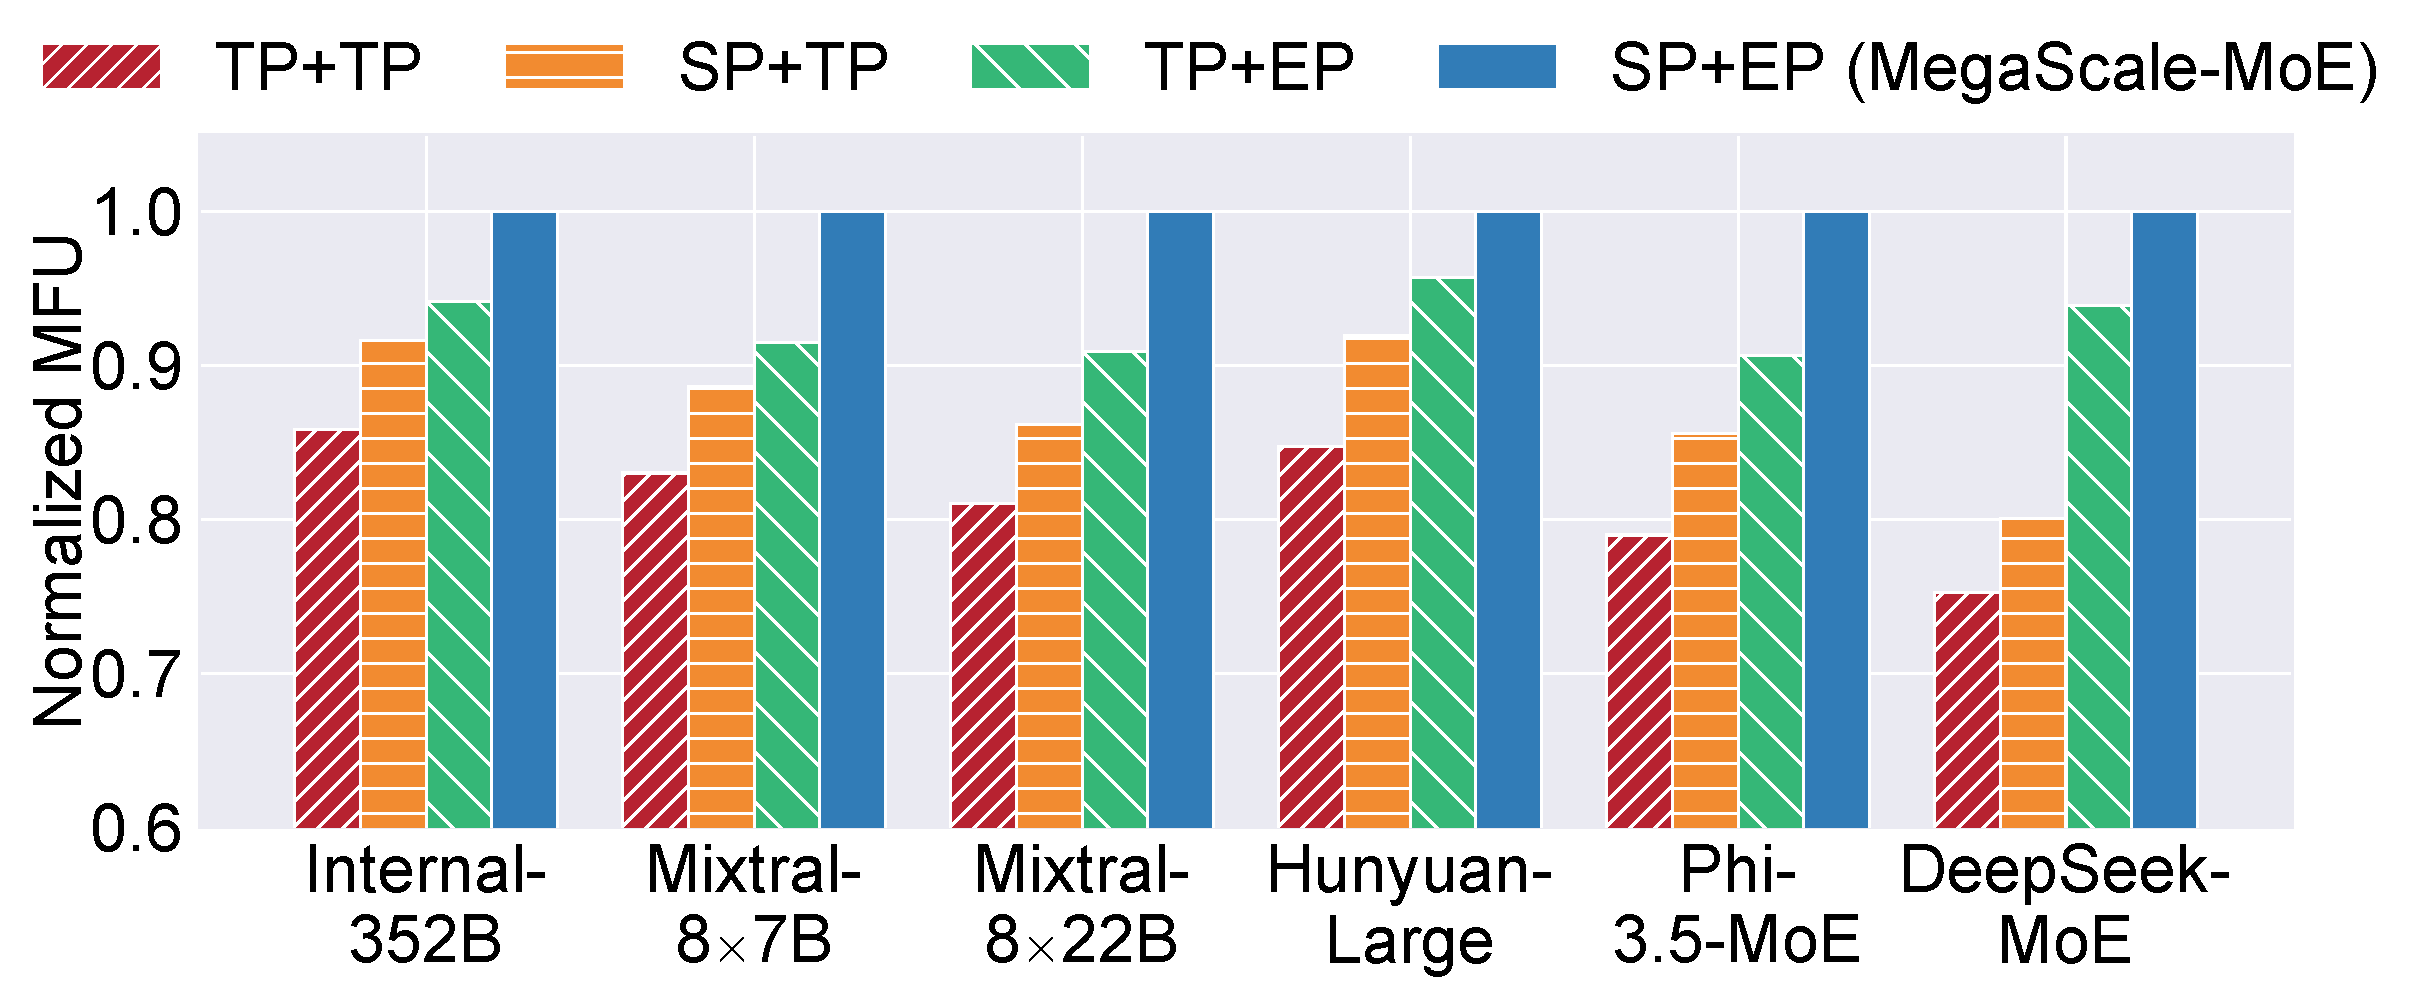
\includegraphics[width=0.8\linewidth]{figures/eval/parallelism_efficiency.pdf}
    \vspace{-0.15in}
    \caption{Parallelism efficiency for different models.}
    \vspace{-0.1in}
    \label{fig:eval:parallelism}
\end{figure}

\begin{figure}[t!]
    \centering
    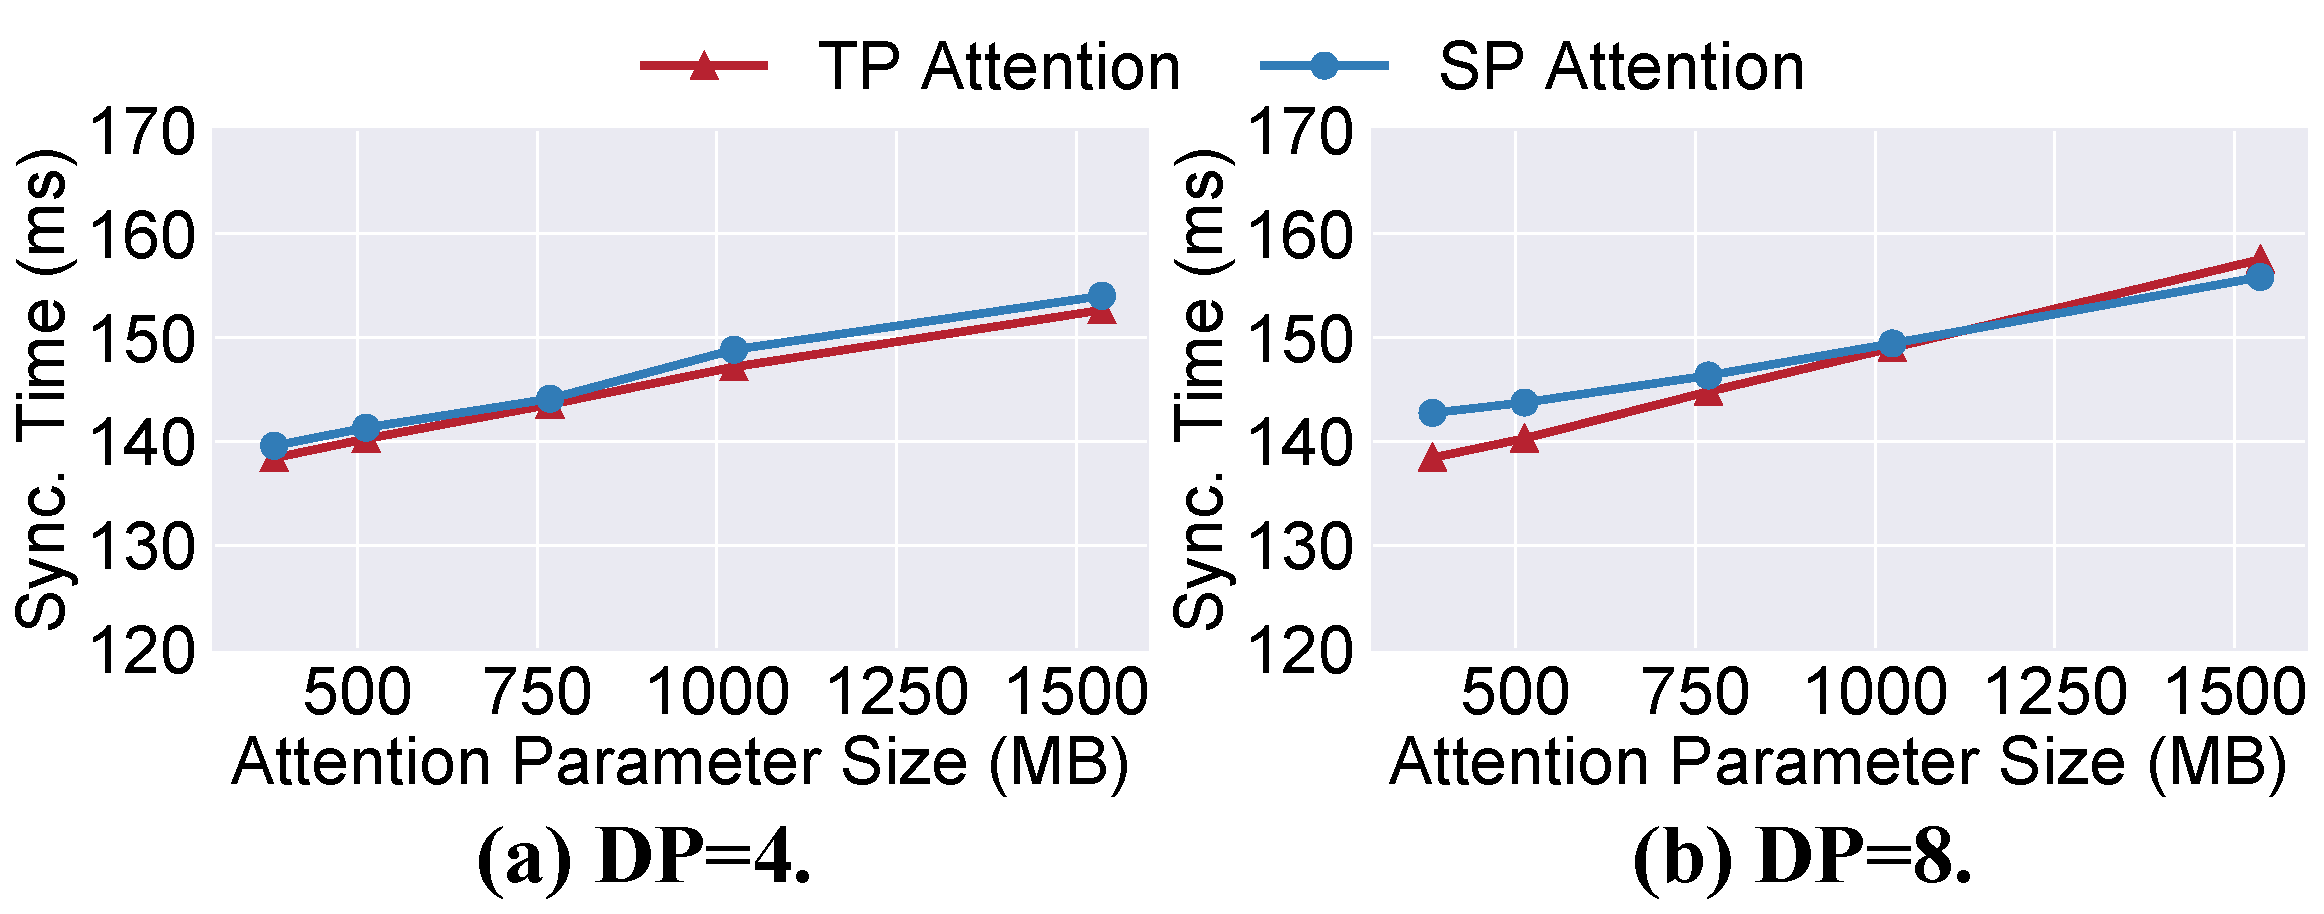
\includegraphics[width=0.9\linewidth]{figures/eval/sync_latency.pdf}
    \vspace{-0.2in}
    \caption{Parameter synchronization time under SP and TP attention.}
    \vspace{-0.1in}
    \label{fig:eval:sync_latency}
\end{figure}

\revision{Following the systematic breakdown, we perform ablation studies on each component, varying a single setting at a time while keeping all others constant, to gain deeper insights into its behavior. }

\begin{figure*}[t!]
    \centering
    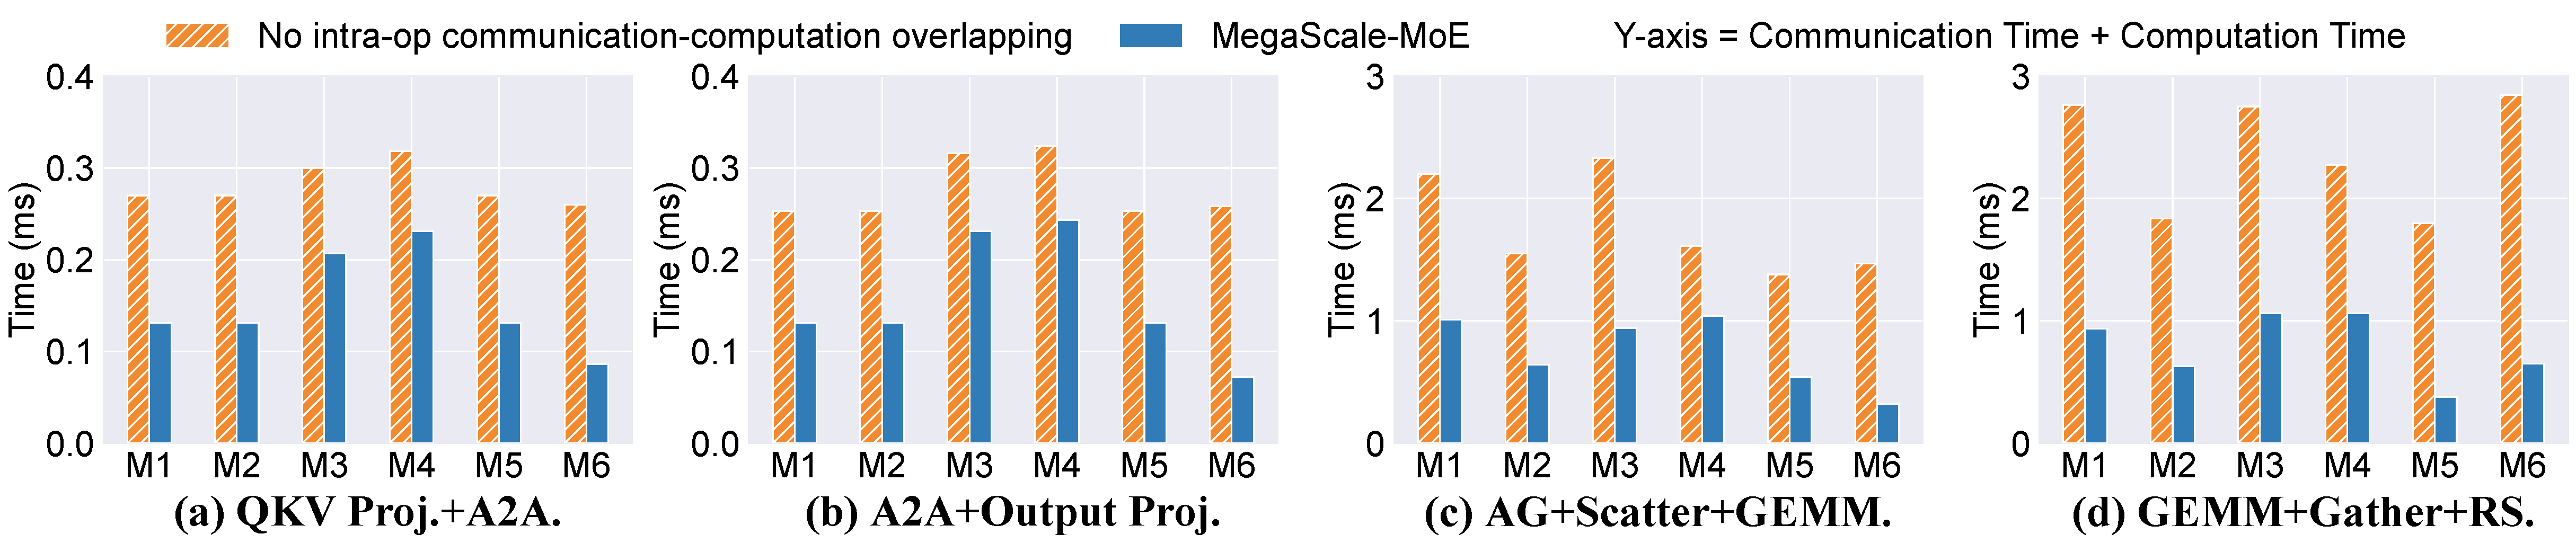
\includegraphics[width=\linewidth]{figures/eval/flux.pdf}
    \vspace{-0.3in}
    \caption{Overlapped communication-computation time vs. non-overlapped time of each layer. M1-M6 represent the six models listed from top to bottom in Table~\ref{tab:evaluation:model_conf}; A2A, AG, and RS refer to all-to-all, all-gather, and reduce-scatter, respectively.}
    \vspace{-0.1in}
    \label{fig:eval:overlapping}
\end{figure*}

\parabf{Parallelism strategy.} We compare the training efficiency under various intra-node parallelism strategies using a single node with eight NVIDIA H800-SXM GPUs. We denote parallelism strategies as X+Y, where X represents the parallelism strategy for attention, and Y corresponds to that for experts. The available parallelism strategies for attention include TP and our SP, whereas for experts, the choices are TP and EP. To isolate the performance benefits of optimized parallelism, we disable other system optimizations. 

\begin{figure}[t!]
    \centering
    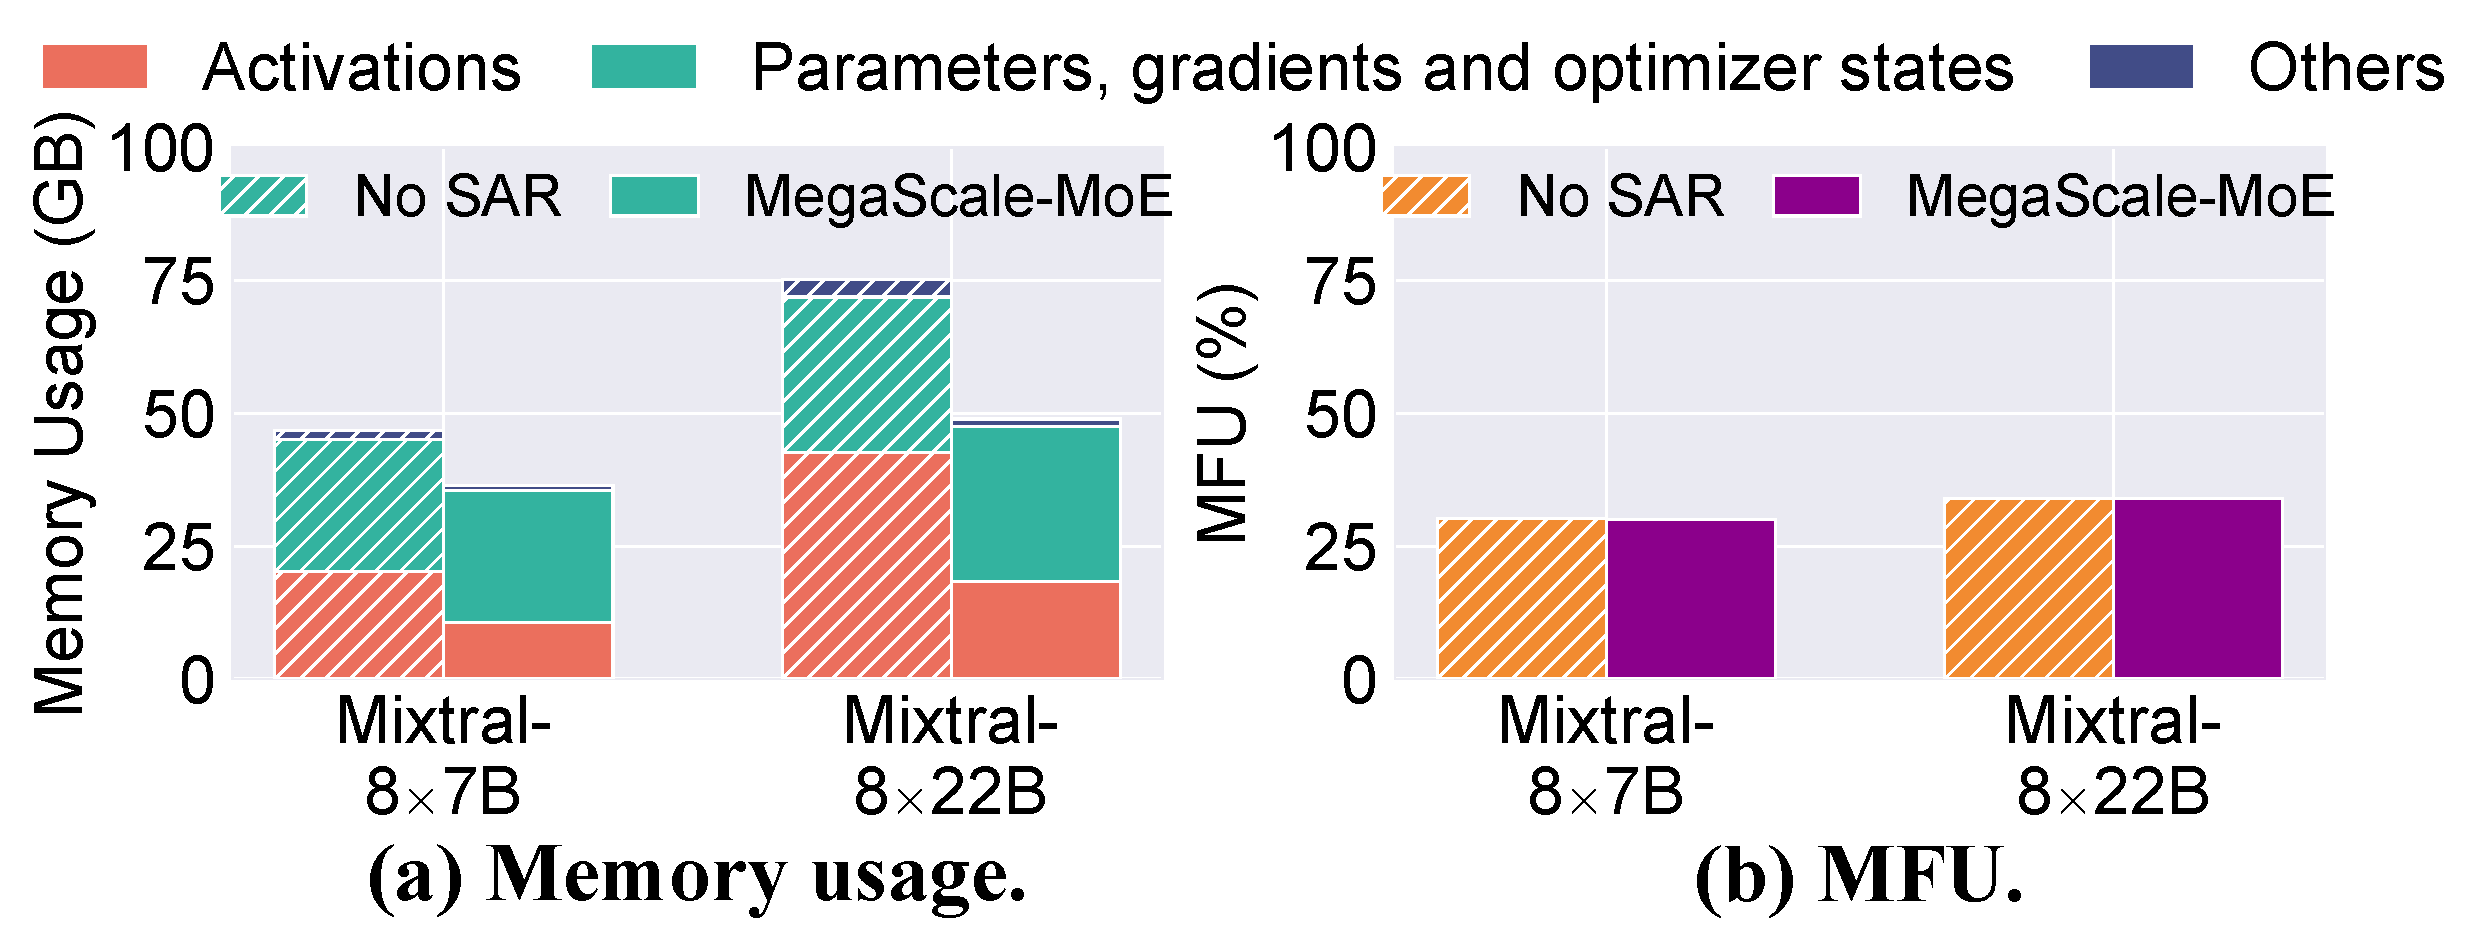
\includegraphics[width=\linewidth]{figures/eval/recomputation.pdf}
    \vspace{-0.3in}
    \caption{Ablation study of selective activation rematerialization (SAR).}
    \vspace{-0.1in}
    \label{fig:eval:recompute}
\end{figure}

We measure the training MFU of one internal and five open-source MoE models with diverse model configurations as listed in Table~\ref{tab:evaluation:model_conf}. The global batch size is set to 32, and we adjust the number of layers for each model to fit within the GPU memory. Figure~\ref{fig:eval:parallelism} shows that \sysname's parallelism strategy, SP+EP, consistently outperforms the other three parallelism strategies, achieving 14.9\%-32.9\% higher MFU compared to TP+TP. The performance gains are attributed to two main factors. 
First, as discussed in \S\ref{sec:design:parallelism}, SP and EP effectively reduce the communication volume compared to TP, thereby decreasing communication overhead. Second, TP partitions the FFN module along the intermediate size dimension, which results in lower GEMM efficiency. 

To provide a more comprehensive evaluation of the parallelism strategy, we also report the additional overhead introduced by the replicated attention parameters in SP. In terms of memory usage, SP incurs a 1.2\%--5.4\% higher memory footprint compared to TP, requiring 1.7\%--8.1\% more memory to store parameters, gradients, and optimizer states across all seven models. This overhead is manageable considering the significant performance gains achieved by SP. 
% Besides, in large-scale training with pipeline parallelism, activation memory constitutes a substantial portion of the overall memory footprint, which reduces the impact of replicated attention parameters.

For the parameter synchronization time, we follow large-scale training setups and set the size of the TP or SP to 8, effectively parallelizing each layer within a single node. 
The attention parameter size on each GPU is varied from 384 MB to 1536 MB, while the FFN parameter size is fixed at 10 GB per GPU, reflecting typical real-world training setups. 
We run \sysname with SP and TP attention, using 4 and 8 DP groups, which correspond to a total of 32 and 64 GPUs, respectively.
Figure~\ref{fig:eval:sync_latency} shows that the synchronization times for SP and TP attention are consistently comparable, differing by only 0.3\%--3.1\%. This aligns with our hypothesis that SP and TP would exhibit similar performance characteristics in DP communication latency.

\parabf{Intra-operator commmunication overlap.} We then measure the duration of four key communication and the corresponding computation operators in the forward pass: $(i)$ QKV Projection paired with all-to-all, $(ii)$ all-to-all with Output Projection, $(iii)$ all-gather with scatter and GroupedGEMM, and $(iv)$ GroupedGEMM with gather and reduce-scatter, as depicted in Figure~\ref{fig:moe_computation}. Figure~\ref{fig:eval:overlapping} demonstrates that across all six models, \sysname achieves a 1.2–4.7$\times$ reduction in the combined time of communication and computation operators compared to the baseline lacking fine-grained overlap. And \sysname reduces the training iteration time by 7.1\%-12.9\% due to intra-operator communication-computation overlap.

\begin{figure}[t!]
    \centering
    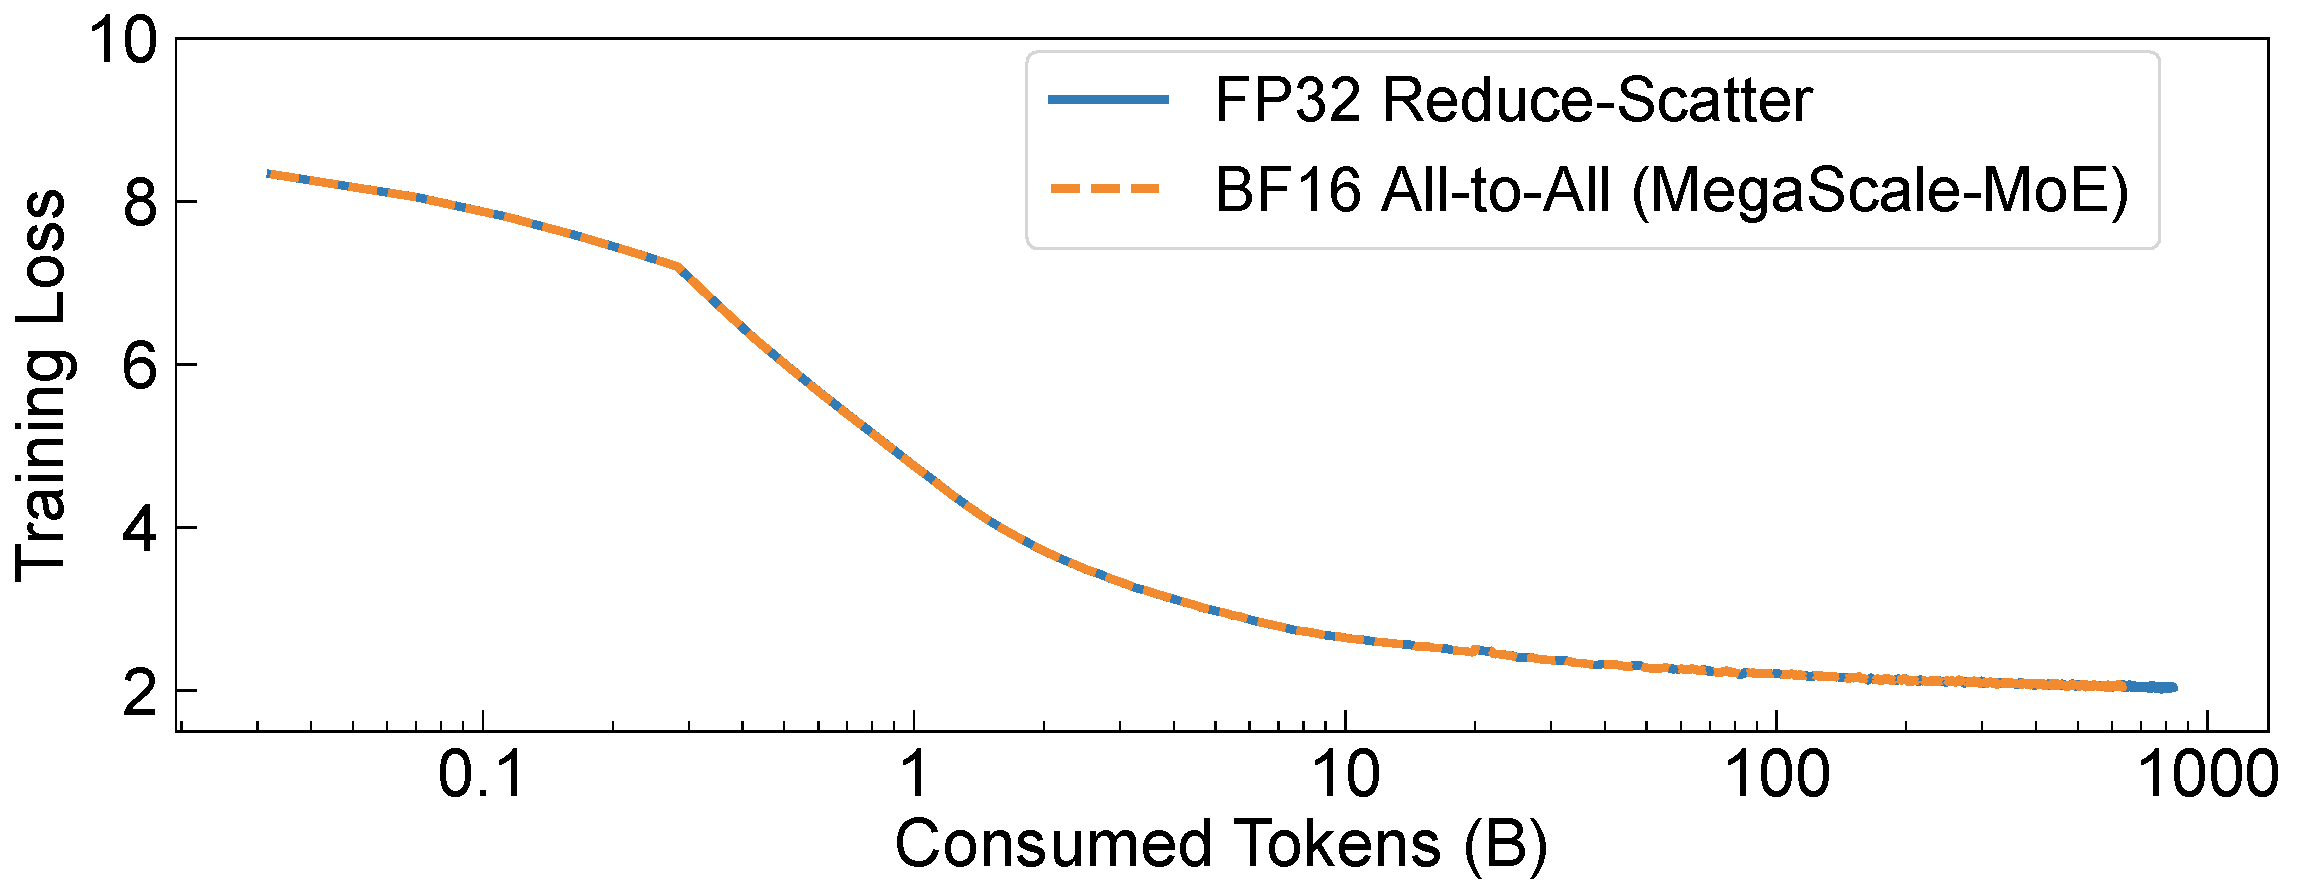
\includegraphics[width=0.8\linewidth]{figures/eval/dp_comm_compression.pdf}
    \vspace{-0.1in}
    \caption{The training loss curve of \sysname with DP communication compression.}
    \vspace{-0.1in}
    \label{fig:eval:bf16_a2a}
\end{figure}

\parabf{Selective activation rematerailization.} We compare \sysname to a baseline that disables selective activation rematerialization (No SAR), which stores all activations in GPU memory during training. We evaluate both methods by training Mixtral-8$\times$7B and Mixtral-8$\times$22B on 128 NVIDIA H800 GPUs. Figure~\ref{fig:eval:recompute} shows the memory usage breakdown and the training MFU. Compared to No SAR, \sysname reduces activation memory consumption by 45.5\% and 57.2\% for the two models, respectively, resulting in overall memory reductions of 21.3\% and 35\%, while maintaining the training performance difference within 0.5\%.

\parabf{Data parallelism communication compression.} We validate the effectiveness of our communication compression technique by training a 7B MoE model using BF16 all-to-all DP communication and FP32 reduce-scatter communication, as described in \S\ref{sec:design:precision}. Figure~\ref{fig:eval:bf16_a2a} illustrates the training loss curves, which are nearly identical. This optimization compresses only the accumulated gradients of the batch and performs conversions between BF16 and FP32 exclusively during communication, introducing minimal risk. 

\subsection{Model Convergence}
\label{sec:evaluation:co-design}

% We evaluate model convergence with our communication compression techniques. Figure~\ref{fig:eval:bf16_a2a} compares the training loss curves of \sysname using BF16 all-to-all DP communication and FP32 reduce-scatter communication. The two curves are nearly identical, as this optimization only compresses the gradients of the final micro-batch, posing minimal risk.
% We also validate the effectiveness of FP8 communication compression by training a 25B MoE model from scratch and continuing training a 100B MoE model from a checkpoint, with their loss curves shown in Figure~\ref{fig:eval:fp8}. With communication compression and optimizations such as tailored activation quantization, \sysname maintains convergence stability and achieves training loss consistent with the BF16 baseline.

We evaluate model convergence with \sysname. Figure~\ref{fig:eval:fp8} demonstrates the loss curves of training a 35B MoE model from scratch and continuing training a 176B MoE model from a checkpoint, with results shown for both BF16 and FP8 precision. \sysname ensures stable convergence and consistent training loss across BF16 and FP8 formats.

\begin{figure}[t!]
    \centering
    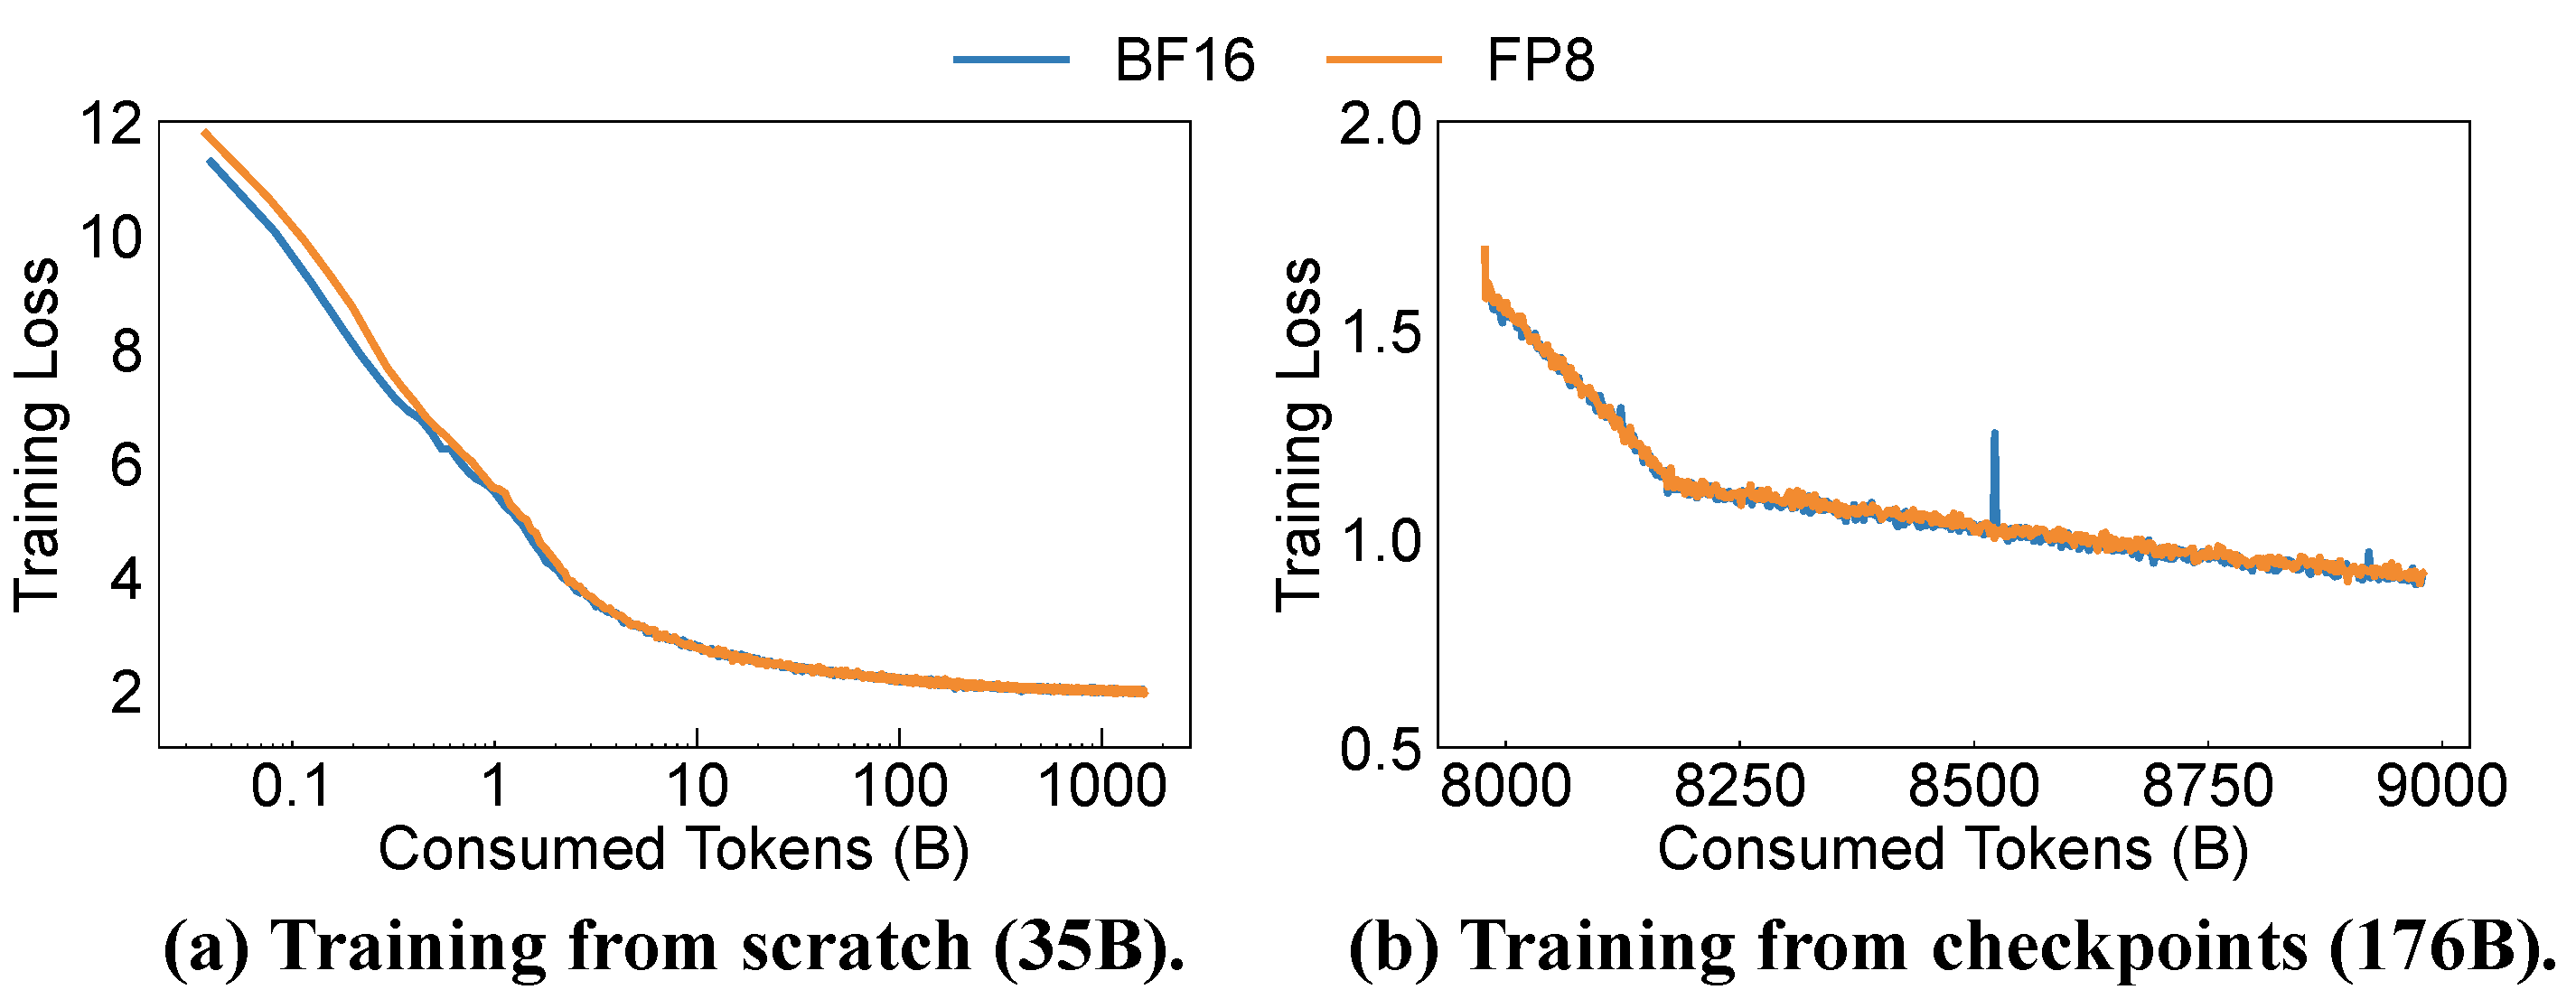
\includegraphics[width=\linewidth]{figures/eval/fp8_comparison.pdf}
    \vspace{-0.2in}
    \caption{The loss curve of \sysname in FP8 and BF16.}
    \vspace{-0.1in}
    \label{fig:eval:fp8}
\end{figure}